\section{Integrace}
\subsection{Určitý integrál pomocí přímé metody}
\begin{equation}
\int_{a}^{b}f(x)\,dx = \Bigr[ F'(x) \Bigr]_a^b=F(b)-F(a)
\end{equation}

\begin{enumerate}
  \item Převést na primitivní funkci
    \begin{itemize}
      \item rozdělit zlomek na dva (o stejném jmenovateli)
    \end{itemize}
  \item Integrace (abych se zbavil $F'(x)\rightarrow$ negace)
  \item Dosadit $\rightarrow$ budu mít 2 funkce
  \item Odečíst
\end{enumerate}

\subsection{Určitý integrál pomocí substituce}
\begin{itemize}\item pro složené funkce\end{itemize}
\begin{align*}
  \int_a^bf(g(x))*g'(x)\,dx&=
  \Biggr|
    \begin{alignedat}{2}
      g(x) &=t \quad &a \rightarrow g(a) \\
      g'(x)\,dx &=\,dt \quad &b \rightarrow g(b) \\
    \end{alignedat}
  \Biggr| = \\
  \text{I. způsob} &= \int_{g(a)}^{g(b)}f(t)\,dt = \Bigr[F(t)\Bigr]_{g(a)}^{g(b)} = F(g(b))-F(g(a)) \\
  \text{II. způsob} &= \int_?^?f(t)\,dt=\Bigr[F(t)\Bigr]_?^? = \\
  &=\Bigr[F(t)\Bigr]_a^b = F(b)-F(a) \\
  & \text{zde existuje mez, vrátím substituci}
\end{align*}

\subsection{Diferenciální rovnice}
\begin{enumerate}
  \item Převést na formu y=...
  \item Přepsat y $\rightarrow\frac{dy}{dx}$
  \item Vynásobím L a P rovnici "dx"
\end{enumerate}

\begin{align*}
  y'=f(x)*g(x)=\frac{dy}{dx}\\
  y'=\frac{dy}{dx}\\
\end{align*}
\begin{center}
    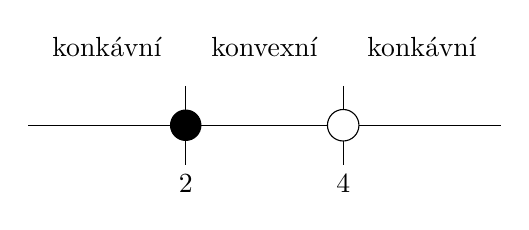
\begin{tikzpicture}[scale=1]
    \draw (-0,0)-- (6,0); %Axis
    \foreach \x in {2,4} {
        \draw (\x,0.5) -- (\x,-0.5) node[below] {\x};
    }
    \fill (2,0) circle (0.2);
    \draw[fill=white] (4,0) circle (0.2);
    % \draw[decorate, decoration={brace}, yshift=2ex] (0,2) -- node{hello} (0,0);
    \draw (1,1) node{konkávní};
    \draw (3,1) node{konvexní};
    \draw (5,1) node{konkávní};
    \end{tikzpicture}
\end{center}
